% !TeX root = ../translation.tex

\section{最优传输理论}

在本章中,我们将介绍经典OT理论中的基本概念
和定理,重点介绍Brenier方法及其在离散集中的推广。具体细节可参考Villani的专著[5]。

\subsection{Monge问题}

假设 $X \subset \mathbb{R}^d, Y \subset \mathbb{R}^d $ 是 $ d $ 维欧几里得空间 $ \mathbb{R}^d $ 的两个子集,$\mu$ 和 $\nu$分别是定义在 $X$ 和 $Y$ 上的两个概率测度,密度函数如下:
\begin{equation*}
	\begin{array}{c} 
		\mu(x) =f(x)dx \\ 
		\nu (y) =g(y)dy 
	\end{array}
\end{equation*}

假设总测度相等,$\mu(X)=\nu(Y)$;即
\begin{equation}
	\int_X f(x)dx =\int_Y g(y)dy
	\label{function:1}
\end{equation}

我们只考虑保测度的映射。

\begin{definition}[保留测度映射]	\label{def:3.1}
	如果映射 $T: X \to Y $ 对于任何可测集合$B \subset Y $,集合 $T^{-1}(B)$ 是 $\mu$- 可测量的,并且 $µ[T^{-1}(B)]=\nu(B)$,那么映射$T: X \to Y$是保测度的,即
	\begin{equation}
		\int_{T^{-1}(B)} f(x)dx =\int_B g(y)dy
		\label{function:2}
	\end{equation}

	测度保持条件记为$T_{\# \mu}=\nu$,其中$T_{\#\mu}$ 是由$T$诱导的前推测度。
\end{definition}

给定一个成本函数 $c(x,y): X \times Y \to \mathbb{R} $,它表示将每个单位质量从源移动到目标的成本,映射$T: X \to Y$的总传输成本被定义为
\begin{equation}
	C_t=\int_X c[x,T(x)]d\mu (x) 
	\label{function:3}
\end{equation}

Monge的OT问题来自于找到使总运输成本最小化的保测度映射。

\begin{problem}[Monge【43】;MP]	\label{problem:3.1}
	给定传输成本函数$c(x,y): X \times Y\to\mathbb{R}_{\ge 0}$,找到保测度映射 $X \to Y$,使总传输成本最小化:
	\begin{equation}
		(MP) \quad \underset{T_{\# \mu}=\nu}{min} \int_X c[x,T(x)]d\mu(x)  
		\label{function:4}
	\end{equation}
\end{problem}

\begin{definition}[OT映射]	\label{definition:3.2}
	Monge问题的解决方案被称为OT映射。一个OT映射的总运输成本被称为$\mu$和$\nu$之间的Wasserstein距离,记为$W_c(\mu,\nu)$。
	\begin{equation}
		W_c(\mu,\nu)= \underset{T_{\# \mu}=\nu}{min} \int_X c[x,T(x)]d\mu(x)  
		\label{function:5}
	\end{equation}
\end{definition}

\subsection{Kontarovich的方法}

根据成本函数及其测度的性质,在$(X、\mu)$和$(Y、\nu)$之间的OT映射可能不存在。Kontarovich将传输映射扩展为传输方案,并定义了联合概率测测度$\rho(x,y): X \times Y \to \mathbb{R}_{\ge 0}$,使$\rho$的边缘概率分别等于$\mu$和$\nu$。令投影映射形式化为$\pi_x(x,y)=x, \pi_y(x,y)=y$,然后定义联合测度类如下:
\begin{equation}
	\Pi(x,y)= \left\{ \rho(x,y): X\times Y \to \mathbb{R} : (\pi_x)_{\#}\rho=\mu, (\pi_y)_{\#}\rho=\nu \right\} 
	\label{function:6}
\end{equation}

\begin{problem}[Kontarovich;KP]	\label{problem:3.2}
	给定一个传输成本函数$c(x,y): X \times Y\to\mathbb{R}_{\ge 0}$,找到保测度映射 $X \to Y$,使总传输成本最小化:
	\begin{equation}
		(KP) \quad W_c (\mu,\nu)= \underset{\rho \in \Pi(\mu,\nu)}{min} \int_{X \times Y} c(x,y)d\rho(x,y)  
		\label{function:7}
	\end{equation}
\end{problem}

Kontarovich问题(KP)可以用LP方法来求解。由于LP等式的对偶性,因此 Eq.(\ref{function:7})(KP方程)可以重新表述为对偶性问题(DP),如下:
\begin{problem}[对偶;DP]	\label{problem:3.3}
	给定一个传输成本函数$c(x,y):X\times Y \to \mathbb{R}_{\ge0}$,找到使总运输成本最小化的联合概率测度$\rho(x,y): X \times Y \to \mathbb{R}_{\ge0}$
	\begin{equation}
		(DP) \quad \underset{\varphi , \psi }{max}\left [ \int_X \varphi (x)d\mu + \int_Y \psi (y)d\nu : \varphi(x)+\psi(y) \ge c(x,y) \right ]   
		\label{function:8}
	\end{equation}
	等式(\ref{function:8})的最大值给出了Wasserstein距离。现有的WGAN模型大多是基于$L^1$代价函数下的对偶公式。
\end{problem}

\begin{definition}[c-转换]	\label{definition:3.3}
	$\varphi: X\to \mathbb{R}$ 的c-变换被定义为$\varphi ^ c: Y \to \mathbb{R}$ :
	\begin{equation}
			\varphi ^c(y)= \underset{x \in X }{inf}\left [ c(x,y)-\varphi(x) \right ]
		\label{function:9}
	\end{equation}
	   
	然后,DP可以重写如下:
	\begin{equation}
		(DP) \quad W_c(\mu , \nu) = \underset{\varphi }{max} \int_X \varphi (x)d\mu +\int _Y \varphi ^c (y)d\nu
		\label{function:10}
	\end{equation}
\end{definition}

\subsection{Brenier方法}

对于二次欧氏距离代价,用Brenier[44]证明了OT映射的存在性、唯一性和内在结构
\begin{theorem}[Brenier【44】]	\label{theorem:3.1}
	假设$X$和$Y$是欧几里得空间$\mathbb{R}^d$的子集,运输代价是欧氏距离的平方$c(x,y)=\frac{1}{2}\left \| x-y \right \| ^2 $。此外,$\mu$是绝对连续的,$\mu$和$\nu$存在有限的二阶矩
	\begin{equation}
		\int _X \left \| x \right \| ^2 d\mu(x) + \int _Y \left \| y \right \| ^2 d\nu(x) < \infty 
		\label{function:11}
	\end{equation}
	
	然后存在一个凸函数$\mu : X \to \mathbb{R}$,即所谓的Brenier势能,其梯度映射 $\bigtriangledown u$ 给出了Monge问题的解:
	\begin{equation}
		(\bigtriangledown u)_{\#} \mu = \nu
		\label{function:12}
	\end{equation}

	 Brenier势能是常熟范围内唯一不变的;因此,最佳的传输映射是唯一的。
	 
	 假设Briener势是$C^2$光滑的,那么它就是以下Monge–Ampère方程的解:
	 \begin{equation}
	 	det(\frac{\partial ^2 u(x)}{\partial x_i \partial x_j})=\frac{f(x)}{g \circ \bigtriangledown u(x)}
	 	\label{function:13}
	 \end{equation}
 
	对于 $\mathbb{R}^d$ 中的$L^2$运输成本 $c(x,y)=\frac{1}{2} \left \| x-y \right \|^2  $,c-变换和经典 Legendre变换具有特殊的关系。
\end{theorem}

\begin{definition}[Legendre变换]	\label{definition:3.4}
	给定一个函数$\varphi : \mathbb{R}^n \to \mathbb{R}$,其Legendre变换定义如下:
	\begin{equation}
		\varphi ^*(y)=\underset{x}{sup}\left [ \left \langle x,y \right \rangle -\varphi (x) \right ]  
		\label{function:14}
	\end{equation}

	当$c(x,y)=\frac{1}{2} \left \| x-y \right \| ^2 $可以证明,以下关系成立:
	\begin{equation}
		\frac{1}{2}\left \| y \right \|^2-\varphi ^c (y)=\left [ \frac{1}{2} \left \| x \right \| ^2-\varphi (x) \right ]^*  
		\label{function:15}
	\end{equation}
\end{definition}

\begin{theorem}[Briener极分解【44】]	\label{theorem:3.2}
	假设$X$和$Y$是欧几里得空间$\mathbb{R}^d$,$\mu$是绝对连续的Lebesgue测度,和映射$\varphi : X\to Y$前推$\mu$为$\nu$,即$\varphi _{\#}\mu=\nu$,然后存在一个凸函数$u: X \to \mathbb{R}$,这样$\varphi=\bigtriangledown u(x)\circ s $ ,在$s: X \to X$是保测度的,$s_{\#}\mu=\mu$。此外,这个分解是唯一的。
\end{theorem}

以下定理在OT理论中是众所周知的
\begin{theorem}[Villani【44】]	\label{theorem:3.3}
	给定紧凸区域$\Omega \subset \mathbb{R}^d$的$\mu$和$\nu$,对于代价$c(x,y)=h(x-y)$存在一个OT方案$\rho$,且$h$严格凸。它是唯一的,并且形式为$(id,T_{\#})\mu \quad$ (id:恒等映射),前提是$\mu$是绝对连续的,而$\partial \Omega$可以忽略不计。此外,存在Kantorovich势能$\varphi$,$T$可以表示为:
	\begin{equation*}
		T(x)=x-(\bigtriangledown h)^{-1} \left [ \bigtriangledown \varphi (x) \right ] 
	\end{equation*}

	当$c(x,y)=\frac{1}{2} \left \| x-y \right \|^2 $,我们有
	\begin{equation*}
		T(x)=x- \bigtriangledown \varphi (x)= \bigtriangledown \left [ \frac{1}{2} \left \| x \right \| ^2 - \varphi(x) \right ] =  \bigtriangledown u(x)
	\end{equation*}

	在这种情况下, Brenier势在$\mu$和Kantorovich势在$\varphi$有以下关系:
	\begin{equation}
		u(x)=\frac{1}{2} \left \| x \right \| ^2 -\varphi (x)
		\label{function:16}
	\end{equation}
\end{theorem}

\subsection{OT映射的正则性}

设$\Omega$和$\Lambda$是$\mathbb{R}^d$上的两个有界光滑开集,设$\mu=fdx$和$\nu=gdy$是该$\mathbb{R}^d$上的两个概率测度$f\mid _{\mathbb{R}^d \setminus \Omega }=0$ 和 $g\mid _{\mathbb{R}^d \setminus \Lambda }=0$。假设$f$和$g$在$\Omega$和$\Lambda$上分别有界远离零和无穷大。

\subsubsection{凸目标域}

\begin{definition}[Hölder连续]\label{definition:3.5}
	一个实值函数或复值函数$f$在$d$维Euclidean空间中满足Hölder条件,或者它是Hölder连续时,此时存在非负实常数$C$,且$\alpha>0$,使得$\left | f(x)-f(y) \right | \le C \left \| x-y \right \|^{\alpha }$对于f定义域中的所有$x$和$y$都成立。。
\end{definition}

\begin{definition}[Hölder空间]	\label{definition:3.6}
	Hölder空间为$(C^{k,\alpha}(\Omega)$,其中$\Omega$是某个Euclidean空间的一个开子集,并且整数$k \ge 0$,它是由在$\Omega$上有直到$k$阶连续偏导数的函数组成,从而使得$k$阶偏导数是$\alpha$阶Hölder连续的,且$0<\alpha \ge 1$。$C_{loc} ^{k,\alpha} (\Omega)$意味着上述条件适用于$\Omega$的任意紧子集。
\end{definition}

\begin{theorem}[Caffarelli【45】]	\label{theorem:3.4}
	如果$\Lambda$是凸的,那么Brenier势$u$是严格凸的;此外,
	
	(1) 如果$\lambda \ge f, g \ge \frac{1}{\lambda}$当$\lambda>0$,则$u \in C_{loc} ^{1,\alpha} (\Omega)$ 。
	
	(2) 如果$f \in C_{loc} ^{k,\alpha} (\Omega)$ 和 $g \in C_{loc} ^{k,\alpha} (\Lambda)$ 对于$f,g>0$,则$u \in C_{loc} ^{k+2,\alpha} (\Omega)$ 和 $(k \le 0, \alpha \in(0,1))$ 。
\end{theorem}

\subsubsection{非凸目标域}

如果$\Lambda$不是凸的,并且存在光滑的$f$和$g$使得$u \notin C^1 (\Omega)$,那么OT映射$\bigtriangledown u$在奇点上是不连续的。


\begin{definition}[次梯度]\label{definition:3.7}
	给定一个开集$\Omega \subset \mathbb{R}^d$和一个凸函数$u: \Omega \to \mathbb{R}$,对于$x \in \Omega$,$u$在$\mathbf{x}$处的次梯度(次微分)定义如下:
	\begin{equation*}
		\partial u(x)=\left \{ p \in \mathbb{R}^n : u(z) \le u(x) + \left \langle p,z-x \right \rangle , \forall z \in \Omega \right \}    
	\end{equation*}
	
	很明显,$u(x)$是一个闭凸集。几何上,如果$\rho \in u(x)$,那么超平面$l_{x,p}(z)=u(x)+\left \langle p,z-x \right \rangle $在$x$从下面接触$u$;也就是说,在$\Omega$和$l_{x,p}(x)=u(x)$上的$l_{x,p} \le u$,其中$l_{x,p}$是$u$在$\mathbf{x}$上的支撑平面。
	
	如果Brenier势$u$的次梯度$\partial u(x)$包含一个点,那么$u$在$\mathbf{x}$上是可微的。我们根据点的子梯度的维数对点进行分类,并定义集合 $\sum _k (u) =\left \{ x \in \mathbb{R}^d \mid \dim \left [ \partial u(x) \right ] =k  \right \} ,k=0,1,2,\cdots ,d$。
	
	很明显,$\sum _0(u)$是正则点的集合,而$\sum _k(u)$,其中$k>0$,是奇异点的集合。我们还定义了在$\mathbf{x}$处的可达的子梯度如下:
	\begin{equation*}
		\partial _* u(x)=\left \{ \lim_{x \to \infty} \bigtriangledown u(x_k) \mid x_k \in \sum _0, x_k \to x \right \}    
	\end{equation*}

	由此可知,次梯度等于可达次梯度的凸包,即:
	\begin{equation*}
		\partial u(x)=Convex \quad hull \quad \bigtriangledown _* u(x)
	\end{equation*}
\end{definition}

\begin{theorem}[正则性]\label{theorem:3.5}
	设$\Omega$,$\Lambda$是两个有界开集,设在$\Omega$和$\Lambda$之外的两个为零的概率密度$f,g : \mathbb{R}^d \to \mathbb{R} ^+$,并且在$\Omega$和$\Lambda$上分别从零和无穷远处间有界。用$T=\bigtriangledown u: \Omega \to \Lambda$表示由定理(\ref{theorem:3.1})提供的OT映射。然后存在两个相对封闭的集$\sum _{\Omega} \subset \Omega$和$\sum _{\Lambda} \Lambda$与$\sum _{\Omega} = \sum _{\Lambda} =0$,这样$T: \Omega \setminus \sum _{\Omega} \to \Lambda \setminus \sum _{\Lambda}$是某些$\alpha > 0$的$C_{loc}^{0,\alpha}$的同态类。
	
	我们称$\sum_{\Omega}$为OT映射的奇异集$\bigtriangledown u : \Omega \to \Lambda$。图 \ref{fig:5} 说明了奇异集的结构,使用基于定理4.2的算法计算。我们得到的计算结果如下:
	\begin{equation*}
		\sum _0 = \frac{\Omega}{\left \{ \sum _1 \cup \sum _2 \right \}} , \sum _1=\bigcup_{k=0}^{3} \gamma _k, \sum _2=\left \{ x_0,x_1 \right \}    
	\end{equation*}
	
	$x_0$的次梯度,$\partial u(x_0)$,是$\Lambda$的整个内孔,而$\partial u(x_1)$是阴影三角形。对于$\gamma _k (t)$上的每个点,$\partial u \left [ \gamma_k(t) \right ]$是$\Lambda$外的一条线段。$x_1$是$\gamma_1,\gamma_2$和$\gamma_3$的分岔点。$\sum_1$和$\sum_2$上的Brenier势是不可微的,它们上的OT映射$\bigtriangledown u$是不连续的。
\end{theorem}

\begin{figure}[h]
	\centering
	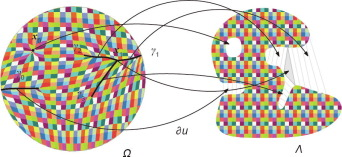
\includegraphics[width=0.6\linewidth]{5.jpg}
	\caption{OT映射的奇异点集结构。}
	\label{fig:5}
\end{figure}